\documentclass[UTF8,12pt,a4paper]{ctexart}

% 使用 Overleaf 时，请把编译器设置为 XeLaTeX。
\usepackage[a4paper,margin=2.5cm]{geometry}
\usepackage{amsmath}
\usepackage{booktabs}
\usepackage{graphicx}
\usepackage{float}
\usepackage{verbatim}
\usepackage[hidelinks]{hyperref}

\setlength{\parindent}{2em}
\linespread{1.35}

\title{基于一元线性回归的气温与冷饮销量关系分析}
\author{姓名：待填写\quad 学号：待填写}
\date{\today}

\begin{document}

\maketitle

\begin{abstract}
本文研究日最高气温与校园冷饮店销量之间的关系。基于连续 15 天的气温和销量数据，首先进行缺失值检查与描述性统计，然后计算 Pearson 相关系数，并建立一元线性回归模型。结果表明，气温与销量呈显著的正相关，相关系数为 0.9985；所建立模型的决定系数为 0.9970，均方根误差为 1.0370 杯。结果说明在当前样本范围内，气温升高通常伴随着冷饮销量增加，且一元线性回归模型具有良好的样本内拟合效果。该模型可以用于辅助短期销量预测与备货决策，但受样本数量较少、影响因素有限等条件约束，结论仍需结合更多数据进一步验证。

\noindent\textbf{关键词：}一元线性回归；Pearson 相关系数；冷饮销量；数据分析
\end{abstract}

\section{问题重述}

某校园冷饮店记录了连续 15 天的日最高气温与冷饮销量。需要利用已有数据分析气温与销量之间的关系，并建立一个简单模型描述两者之间的数量关系。具体任务包括：检查数据质量，计算描述性统计量与相关系数，建立一元线性回归模型，评价模型的拟合效果，并讨论模型的实际意义和局限性。

\section{数据分析与预处理}

\subsection{数据说明}

数据共包含 15 条观测和 3 个字段，其中用于建模的两个主要变量如表~\ref{tab:variables} 所示。另一个字段为观测日序号，用于标识样本顺序，不直接参与回归建模。

\begin{table}[H]
    \centering
    \caption{主要变量及其含义}
    \label{tab:variables}
    \begin{tabular}{ccc}
        \toprule
        变量 & 含义 & 单位 \\
        \midrule
        $x$ & 日最高气温 & $^\circ$C \\
        $y$ & 当日冷饮销量 & 杯 \\
        \bottomrule
    \end{tabular}
\end{table}

\subsection{数据检查}

使用 Python 对数据规模、数据类型和缺失值进行检查。结果显示，日序号、日最高气温和冷饮销量三个字段的缺失值数量均为 0，数据记录完整。同时结合变量的取值范围进行初步检查，气温位于 18 至 32~$^\circ$C 之间，销量位于 82 至 141 杯之间，未发现明显不合理的数据，因此保留全部样本用于后续分析。

\subsection{描述性统计}

气温和销量的描述性统计结果如表~\ref{tab:descriptive} 所示。

\begin{table}[H]
    \centering
    \caption{主要变量的描述性统计}
    \label{tab:descriptive}
    \begin{tabular}{ccccc}
        \toprule
        变量 & 均值 & 标准差 & 最小值 & 最大值 \\
        \midrule
        气温 & 25.000 & 4.472 & 18 & 32 \\
        销量 & 109.867 & 19.467 & 82 & 141 \\
        \bottomrule
    \end{tabular}
\end{table}

由表~\ref{tab:descriptive} 可知，样本期间气温位于 18 至 32~$^\circ$C 之间，冷饮销量位于 82 至 141 杯之间。气温与销量均具有一定的变化范围，可以用于初步分析两个变量之间的数量关系。

\section{模型建立与求解}

\subsection{分析流程}

本文的完整分析流程如图~\ref{fig:workflow} 所示。

\begin{figure}[H]
    \centering
    \IfFileExists{figures/workflow.pdf}{
        \includegraphics[width=0.68\textwidth]{figures/workflow.pdf}
    }{
        \fbox{\parbox[c][5cm][c]{0.72\textwidth}{\centering
        此处插入你用 draw.io 绘制的流程图：\\
        \texttt{figures/workflow.pdf}}}
    }
    \caption{气温与冷饮销量关系分析流程}
    \label{fig:workflow}
\end{figure}

\subsection{相关分析}

采用 Pearson 相关系数衡量气温与销量之间的线性相关程度：

\begin{equation}
    r=\frac{\sum_{i=1}^{n}(x_i-\bar{x})(y_i-\bar{y})}
    {\sqrt{\sum_{i=1}^{n}(x_i-\bar{x})^2}\sqrt{\sum_{i=1}^{n}(y_i-\bar{y})^2}}.
\end{equation}

计算得到 $r=0.9985$。该系数为正且非常接近 1，说明在当前样本中，日最高气温与冷饮销量之间存在很强的正线性相关关系，即较高气温通常对应较高销量。需要指出的是，相关系数只能反映变量之间的统计关联，不能仅凭该结果证明气温变化是销量变化的唯一原因。

\subsection{一元线性回归模型}

以日最高气温 $x$ 为自变量，以冷饮销量 $y$ 为因变量，建立一元线性回归模型：

\begin{equation}
    y_i=\beta_0+\beta_1x_i+\varepsilon_i,
\end{equation}

其中，$\beta_0$ 为截距，$\beta_1$ 为回归系数，$\varepsilon_i$ 为随机误差。使用最小二乘法估计模型参数，得到拟合方程：

\begin{equation}
    \hat{y}=1.2060+4.3464x.
\end{equation}

斜率的实际意义是：在当前数据范围和其他影响因素未被单独控制的条件下，日最高气温每升高 $1\,^{\circ}$C，模型预测冷饮销量平均增加约 4.35 杯。截距表示气温为 $0\,^{\circ}$C 时的形式预测值，但该温度超出本样本的观测范围，因此不宜作过强的实际解释。

\subsection{模型评价指标}

采用决定系数 $R^2$ 和均方根误差 RMSE 评价模型：

\begin{equation}
    R^2=1-\frac{\sum_{i=1}^{n}(y_i-\hat{y}_i)^2}
    {\sum_{i=1}^{n}(y_i-\bar{y})^2},
\end{equation}

\begin{equation}
    \mathrm{RMSE}=\sqrt{\frac{1}{n}\sum_{i=1}^{n}(y_i-\hat{y}_i)^2}.
\end{equation}

$R^2$ 越接近 1，说明模型对样本中销量变化的解释程度越高；RMSE 越小，说明预测值与真实值之间的平均偏差越小。

\section{结果分析}

原始观测数据和回归模型的拟合结果如图~\ref{fig:fit} 所示。

\begin{figure}[H]
    \centering
    \IfFileExists{figures/scatter_fit.pdf}{
        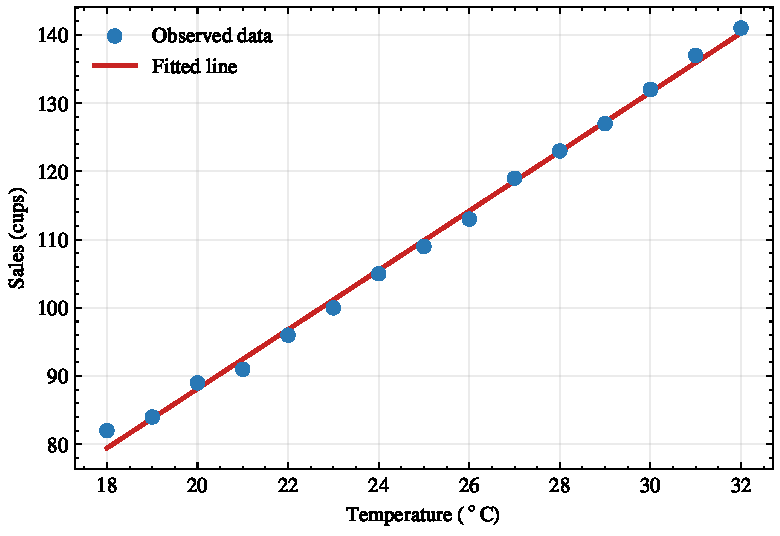
\includegraphics[width=0.78\textwidth]{figures/scatter_fit.pdf}
    }{
        \fbox{\parbox[c][5cm][c]{0.72\textwidth}{\centering
        此处插入 Python 生成的散点图与拟合直线：\\
        \texttt{figures/scatter\_fit.pdf}}}
    }
    \caption{气温与冷饮销量的散点图及线性拟合结果}
    \label{fig:fit}
\end{figure}

由图~\ref{fig:fit} 可知，各观测散点随气温升高呈明显上升趋势，并且整体紧密分布在拟合直线附近，仅存在幅度较小的上下波动。模型的决定系数为 $R^2=0.9970$，说明该线性模型能够解释当前样本中约 99.70\% 的销量变异；RMSE 为 1.0370 杯，表示样本内模型预测值与实际销量之间的典型偏差约为 1.04 杯。综合相关系数、$R^2$ 和 RMSE，可以认为该模型对当前 15 天数据具有良好的线性拟合效果，但仍需使用更多独立数据检验其未来预测能力。

\section{结论与不足}

本文利用 15 天观测数据分析了日最高气温与冷饮销量之间的关系。研究结果表明，两者存在很强的正线性相关关系，拟合方程为 $\hat{y}=1.2060+4.3464x$；在当前样本范围内，气温每升高 $1\,^{\circ}$C，模型预测冷饮销量平均增加约 4.35 杯。模型的 $R^2$ 为 0.9970、RMSE 为 1.0370 杯，表明其样本内拟合误差较小。建立的一元线性回归模型形式简单，能够直观描述气温变化与销量变化之间的数量关系，可为冷饮店的短期备货提供初步参考。

本模型仍存在以下不足：第一，样本数量较少，数据只覆盖 15 天；第二，销量还可能受到降雨、节假日、促销和客流量等因素影响；第三，当前分析得到的是统计相关关系，不能单独证明因果关系。后续可以收集更长时间的数据，并引入其他影响变量建立多元回归或时间序列模型。

\begin{thebibliography}{9}
    \bibitem{numpy}
    Harris C R, Millman K J, van der Walt S J, et al.
    Array programming with NumPy[J]. Nature, 2020, 585: 357--362.
\end{thebibliography}

\appendix
\section{Python 核心代码}

\IfFileExists{analysis.py}{
    \verbatiminput{analysis.py}
}{
    请在此处附上数据分析与绘图代码。
}

\end{document}
